\subsection{Genome Instrumentation}
\label{sec:genome-instrumentation}

This section reviews hereditary stratigraphic annotation methodology as originally developed for inference over asexual populations and introduces the gene- and species-level instrumentation strategies proposed to apply it to sexual populations.
The former strategy is used for positive selection inference and the later is used for genealogical and population size inference.

Subsequent discussion describes recombination and gene drive mechanisms employed for species-level instrumentation and evaluates the extent to which this methodology increases the expected rate of spurious differentia collision, which can lead to overestimation of relatedness from hereditary stratigraph instrumentation.


% \begin{figure}
  \centering
  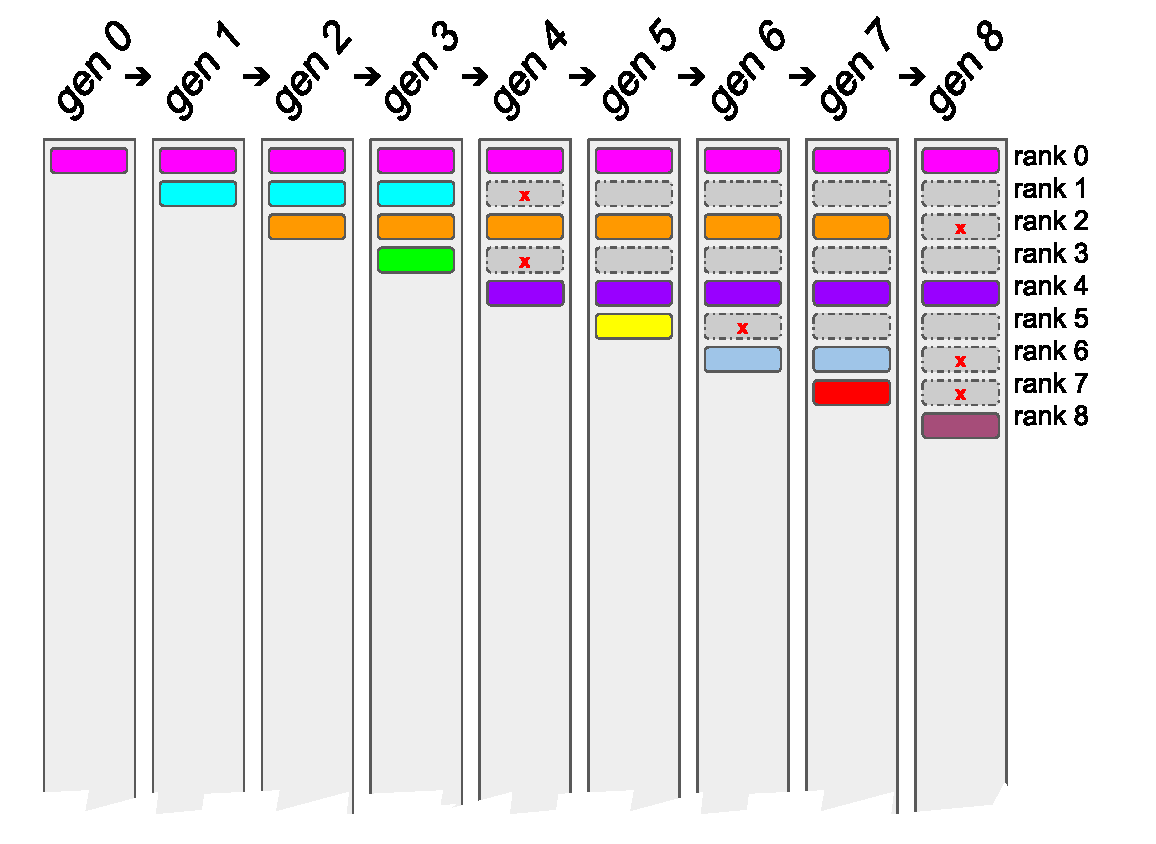
\includegraphics[width=\textwidth]{img/deposit-prune-example}
  \caption{
    TODO
  }
  \label{fig:deposit-prune-example}
\end{figure}

% \begin{figure}
  \centering
  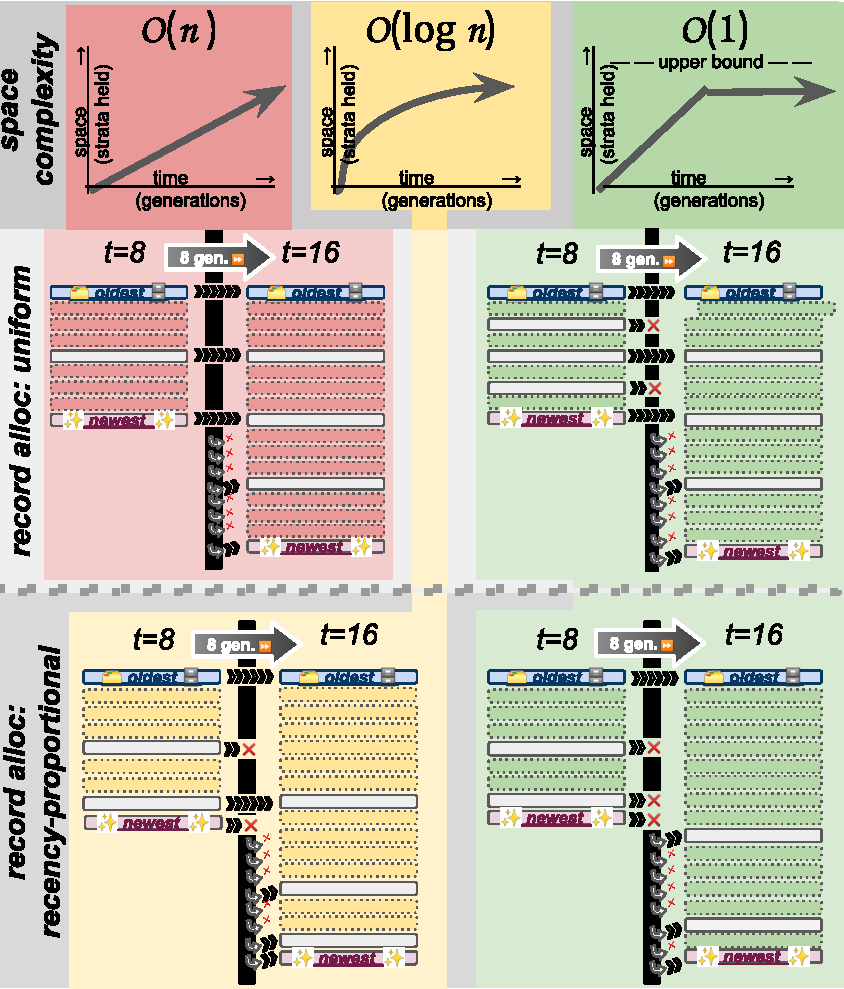
\includegraphics[width=\textwidth]{img/retention-policy-matrix}
  \caption{
    Comparison of four stratum retention policies by space complexity per stratigraph with respect to generations elapsed (columns, red/yellow/green) and by distribution of retained differentia (rows).
    Uniform allocation keeps differentia in evenly-spaced layers.
    Recency-proportional allocation keeps more more-recent differentia, trading off coarser resolution to infer ancient phylogenetic events for finer resolution to infer recent phylogenetic events.
    Retained layers under each policy are shown at $t=8$ generations and $t=16$ generations, with new differentia being deposited in a descending fashion.
    Differentia pruning events are noted with a red $x$.
  }
  \label{fig:retention-policy-matrix}
\end{figure}

\textbf{Hereditary Stratigraphy.}
Proposed methods for genealogical and evolutionary inference over distributed sexual populations draw on ``hereditary stratigraphy'' technique, originally developed to facilitate phylogenetic inference over asexual populations \citep{moreno2022hstrat}.
The core mechanism of this technique is generation-on-generation accumulation of randomized ``fingerprint'' packets.
Offspring inherit parents' fingerprint record and append an entry.
This process repeats with the next generation.

Each accumulated fingerprint ultimately serves as a kind of linealogical checkpoint.
Because fingerprints are faithfully inherited each generation after their creation, discrepancy between coincident fingerprints implies divergent ancestry at their shared time point.
So, the end of common ancestry necessarily precedes the first mismatching fingerprints.

To establish practical viability, some attention must be paid to space complexity.
Proceeding naively, perpetual fingerprint accumulation with each generation would hopelessly bloat memory use.
Fortunately, the underlying inferential mechanism is amenable to thinning out fingerprints within hereditary stratigraph records.
Pruned-away fingerprints introduce a commensurate uncertainty into estimation of two records' divergence generation.
If every other fingerprint was pruned, for example, divergence generations would only be estimable to within 2 generations.
In this way, flexibility in configuring what fingerprints to keep when directly provides for direct administration of the inherent trade-off between annotation memory use and inferential power.
Although beyond present scope, significantly more can be said about this running fingerprint curation process --- the algorithmic core of hereditary stratigraphy.
For detail, refer to \citep{moreno2022hereditary}.

Fingerprint pruning was not performed in the reported experiments in order to simplify experimental setup and analysis, experiments reported here do not incorporate fingerprint pruning.
All inference mechanisms introduced here are, in principle, compatible with fingerprint pruning.
However, further work remains to directly investigate how pruning affects presented approaches' characterization of evolutionary history and dynamics in sexual populations.
Analogous work in asexual populations will provide some initial indications in this direction \citep{moreno2023toward}.

This work uses 64 bit fingerprints, which collide spuriously with negligible probability $1/2^{64} \approx 5 \times 10^{-20}$.
At population size 100 over 200 generations, as in the first sets of reported experiments, the probability of any collision is miniscule, $< 2 \times 10^{-15}$.
At population size 200 over 400 generations, as in the last set of reported experiments, the probability of any collision is also miniscule, $< 5 \times 10^{-15}$.

\begin{SCfigure}[3][b]
  \centering
  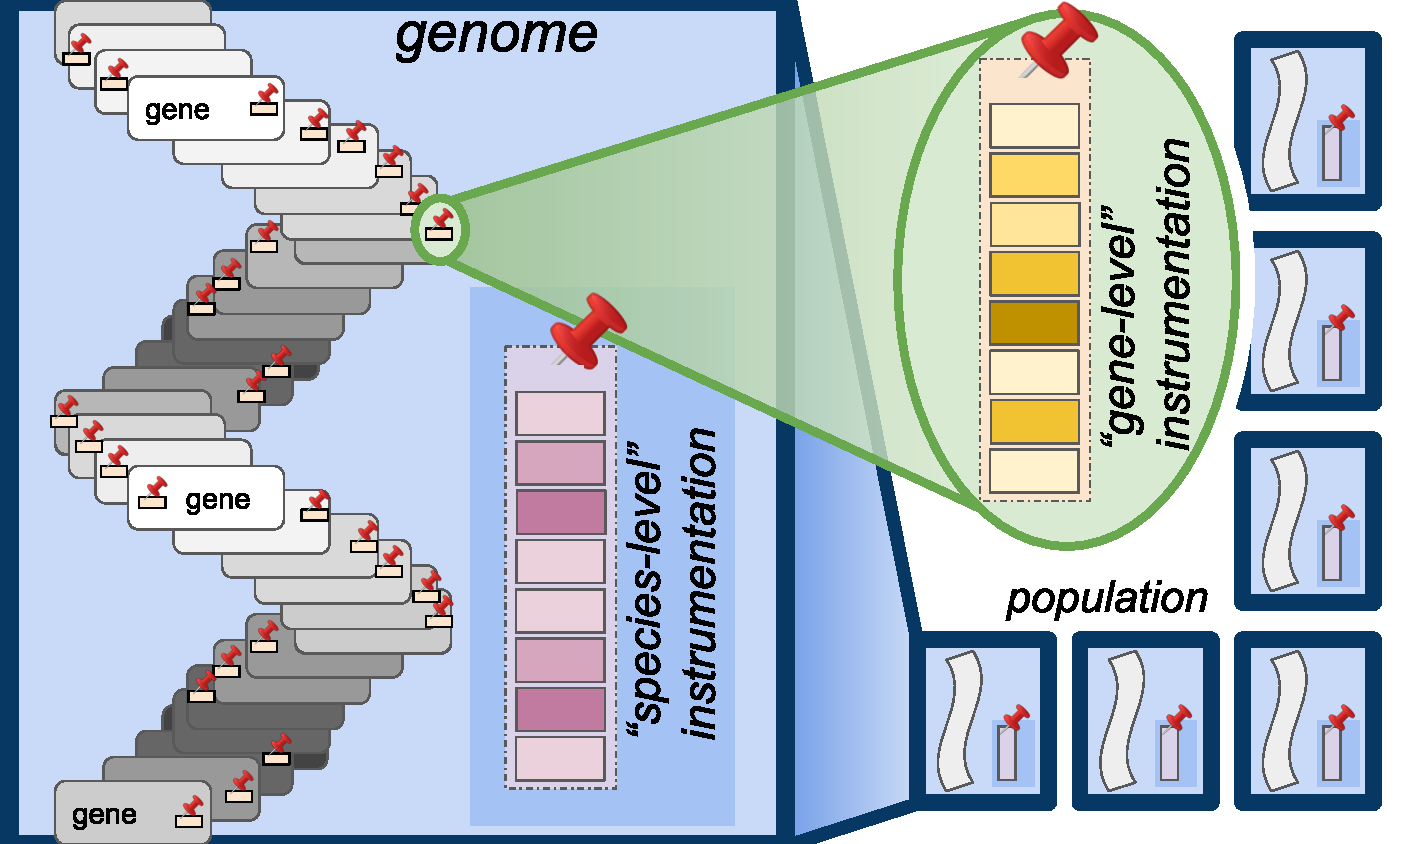
\includegraphics[width=0.5\textwidth]{img/annotation-types}
  \caption{
    Proposed instrumentation methods: ``species-level'' and ``gene-level'' instrumentation.
    Each organism has a single hereditary stratigraph attached as species-level instrumentation, with a gene drive mechanism (Figure \ref{fig:gene-drive}) ensuring consistentcy within species (i.e., interbreeding populations).
    Gene-level instrumentation associates instrumentation with individual genes, to be used for gene tree reconstructions.
  }
  \label{fig:annotation-types}
\end{SCfigure}

\textbf{Sexual Instrumentation Schemes.}
As originally devised for asexual populations, hereditary stratigraphic markers followed a one-to-one relationship to genomes.
Here, we explore two alternate schemes designed for instrumentation of sexual populations: gene instrumentation and species instrumentation.
Figure \ref{fig:annotation-types} compares these two schemes.

The former treats individual genes as asexual subcomponents of sexual lineages, instrumenting genes individually using the original hereditary stratigraphy methodology.
This strategy involves (potentially) several independent hereditary stratigraph instruments per organism.
In, along the lines of ``gene tree'' analsyes in traditional phylogenetics \citep{avise1989gene}.

In cases where digital chromosomes comprise a relatively small number of atomic genes, it may make sense to instrument every gene independently.
However, in applications with very fine atomic genes (e.g., individual GP instructions) or no atomic genes (e.g., GA floating point values subjected to interpolation during crossover) may warrant instrumentation of a representative subset of genes or introduction of ``dummy'' genes associated with certain chromosomal positions.

Species-level instrumentation operates via hereditary stratigraphic columns associated with individual genomes.
Instrumentation consensus within interbreeding populations is achieved through a gene drive mechanism that forces a single consensus differentia value to sweep each hereditary stratigraph layer within interbreeding populations (i.e., species), described below.
Although gene drive mechanisms are widespread in natural systems \citep{alphey2020standardizing, price2020resistance}, unlike gene-level annotation this technique has no direct analogy in traditional phylogenetic analyses.

Species-level instrumentation was employed for genealogical inference and population size inference (Sections \ref{sec:genealogical-inference} and \ref{sec:population-size-inference}).
Gene hereditary stratigraph instrumentation was employed for positive selection inference (Section \ref{sec:selection-inference}).

\begin{SCfigure}[3][b]
  \centering
  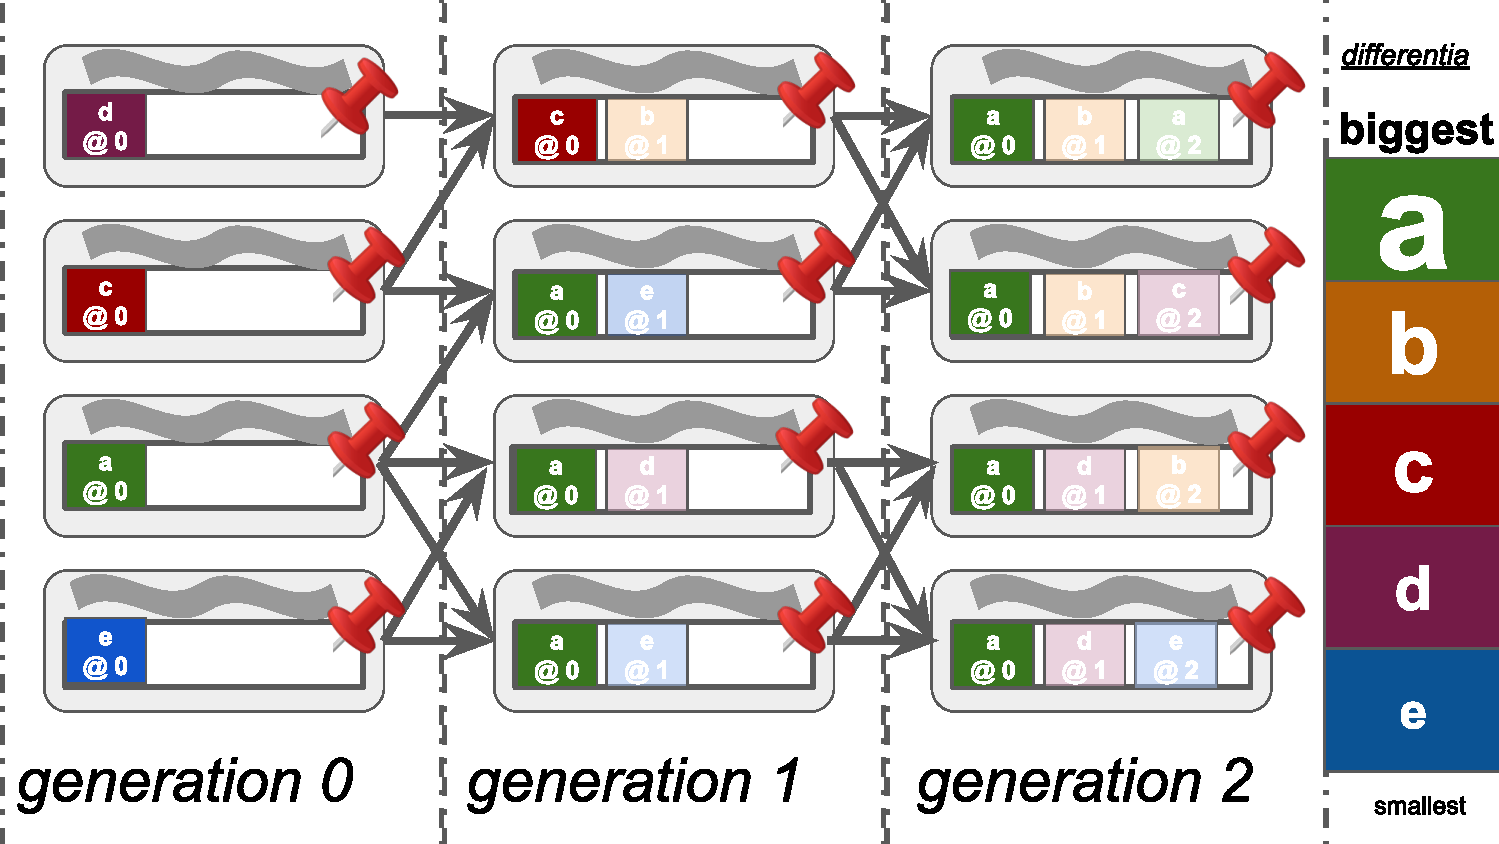
\includegraphics[width=0.6\textwidth]{img/gene-drive}
  \caption{
    Gene drive mechanism for species-level instrumentation.
    The larger of parents' differentia values at each layer is inherited.
    The largest value generated among layer 0 differentia ($a$) spreads from one member at generation 0 to all four by generation 2.
    This mechanism applies to ``species-level'' instrumentation (Figure \ref{fig:annotation-types}).
  }
  \label{fig:gene-drive}
\end{SCfigure}

\textbf{``Gene-drive'' Recombination Mechanism.}
Successful species-level tracking necessitates consistent labeling of interbreeding population members and consensus among members on phylogenetic history.
In the hereditary stratigraphic context, this translates to consistency among corresponding-time point fingerprint differentia values among population members.
Recombination of differentia values between genome instrumentaiton markers will, in the limit, enforce such consensus.
Under such a scheme, offspring would inherit differnetia values at each instrumentation layer independently, with values assigned to the offspring's instrumentation layers chosen arbitrarily from the corresponding layer of either of the parents.
A single consensus fingerprint will eventually fix at each instrumentation layer within the population through drift.
However, expected time to coalescence can be long for large populations.
Further, distributions of coalescence times is fat-tailed, meaning that time for \textit{all} sites to reach consensus would be prohibitively large in most cases.

A simple inheritance rule induces faster consensus: the larger of parents' differentia values at each instrumentation layer is inherited by all offspring.
In well-mixed populations and structured populations with long-distance migration, copy count of the largest-magnitude differentia value will grow rapidly until reaching fixation.
Figure \ref{fig:gene-drive} depicts this mechanism.

Asynchronous generations slightly complicate the picture.
When individuals from different generations recombine, one parent will necessarily have fingerprint layers not present in the other.
How should recombination proceed in this case?
One possibility would be to simply ``fast-forward'' the younger instrument to match the generational depth of the elder.
However, like with fingerprint pruning above, full consideration of asynchronous generations remains for future work.
All reported experiments use synchronous generations.

The described gene drive-based recombination mechanism described in this section only applied exclusively to species-level instrumentation.
(Gene-level instruments, although tagging along with genes shuffled up through genome-level recombination, did not themselves recombine.)

\textbf{Fingerprint Collision Probability.}
Fixed genes' skew toward large-magnitude integers due to the dominance of larger values in gene drive competition increases the probability of fixed-gene collision between two populations causing spurious detection of shared ancestry between the populations.
This collision probability effect presents a potential threat to the efficacy of this approach at scale.
We will assess the extent of this potential problem by computing threshold population sizes where collision becomes substantive.

Suppose independent populations of size $a$ and $b$.
The largest gene in each population will drive to fixation.
If each population members' gene is drawn from uniform distribution on integers $[0, u)$, then the probability of collision between the populations' fixed genes can be derived as

\begin{align*}
\frac{a \sum_{n=1}^{a + b - 1} \frac{u^{- n - 1} \left(\frac{u - 1}{u}\right)^{a + b - n - 1} \left(- \frac{{\binom{a - 1}{n}}}{{\binom{a + b - 1}{n}}} + 1\right) {\binom{a + b}{n + 1}}}{1 - \left(\frac{u - 1}{u}\right)^{a + b - 1}}}{a + b} \\
+ \frac{b \sum_{n=1}^{a + b - 1} \frac{u^{- n - 1} \left(\frac{u - 1}{u}\right)^{a + b - n - 1} \left(- \frac{{\binom{b - 1}{n}}}{{\binom{a + b - 1}{n}}} + 1\right) {\binom{a + b}{n + 1}}}{1 - \left(\frac{u - 1}{u}\right)^{a + b - 1}}}{a + b}.
\end{align*}

% Derivation will be provided in supplementary materials. TODO?

For 32-bit differentia $u = 2^{32}$, collision occurs with $p < 0.5$ ($p = 0.46$) for two populations of size $a = b = 2^{32}$ .
Collision occurs with $p < 0.01$ for two populations of size $a = b = 2^{26}$.
So, 32-bit fingerprints can differentiate species pairs of around$ 6.7 \times 10^{7}$ members each with reasonable consistency.
Reported experiments used 64-bit fingerprint values, which will exhibit even lower collision probabilities.
However, numerical considerations complicate calculation.
